\section{Results}\label{sec:results}

% \ra{1.1}
    {\begin{tabularx}{\textwidth}{lYYYYY} \toprule
         Copula/Asset & $t$ & Plackett & GMI & rotGumbel & NIG \\ \midrule
     \multicolumn{6}{l}{Individual Cryptos}                                                                                 \\
        \ \ \ BTC          & 73         & 4                 & 2                        & 1                  & 31                  \\
        \ \ \ ETH          & 3          & 6                 & 8                        & 94                 & 1                   \\
        \ \ \ ADA          & 0          & 0                 & 0                        & 0                  & 112                 \\
        \ \ \ LTC          & 13         & 0                 & 3                        & 32                 & 64                  \\
        \ \ \ XRP          & 0          & 31                & 3                        & 78                 & 0                   \\
   \multicolumn{6}{l}{Crypto Indices with BTC Constituent}                                                                  \\
        \ \ \ BITX         & 39         & 0                 & 14                       & 16                 & 12                  \\
        \ \ \ CRIX         & 47         & 0                 & 11                       & 3                  & 27                  \\
        \ \ \ BITW100      & 42         & 0                 & 8                        & 29                 & 2                   \\
    \multicolumn{6}{l}{Crypto Indices without BTC Constituent}                                                              \\
        \ \ \ BITW20       & 0          & 0                 & 0                        & 78                 & 3                   \\
        \ \ \ BITW70       & 0          & 0                 & 0                        & 80                 & 1                   \\
    \bottomrule
    \end{tabularx}
        \caption{Copula Selection Results. }










\subsection{Overview}\label{sec:overview}
In general, the hedged portfolio's performance depends on which spot is being hedge,
Risk minimization objectives and copulae are not critical to the results as long as the objective is not
ES 99\% or VaR 99\%, and copula is not Frank or rotGumbel.
We will discuss the hedged portfolios results of different settings in this section.
Figure \ref{fig:overview} present the out-of-sample hedged portfolio returns and the corresponding OHR.
The dates when the five smallest returns occur in the spot return are highlghted in the figure in black vertical lines. \medskip

Overall, the BTC-involved spots, i.e. BTC, CRIX, BITX, and BITW100, are well hedged by the BTCF.
The overall magnitude of the hedged portfolio returns are greatly reduced, as well as the extreme losses in spot are no longer the extreme losses in the hedged portfolio returns.
Most of the time different risk reduction objectives generate very similar hedged portfolio returns.
As the result hedged portfolio returns are overlapping to each other. \medskip

The OHRs of these portfolios are close to one regardless of which risk minimization objective is taken.
Let's look at the BTC-BTCF portfolio first.
It is natural for the OHRs of the BTC-BTCF close to one as the futures price $F$ is governed by the underlying price $S$ and interest rate $r$
$$F = Se^{rT},$$
where $T$ is the futures' time to maturity.
It s not difficult to show that the arithmetic difference between the daily log returns is almost zero, i.e. $\log\frac{F_{t+1}}{F_t} \approx \log\frac{S_{t+1}}{S_t}$.
This relationship explains every OHRs in BTC-BTCF portfolio are close to one. \medskip

Most of the time the OHRs in the BTC-BTCF portfolio are steady and well-performing,
but we can find fluctuations in MES99\%HR and MVaR99\%HR.
In particular, MES99\%HR fluctuates greatly from Jun 2019 to Aug 2019.
The MES99\%HR is lower than its counterparts and so the resulting hedge fail to capture the magnitude of the negative return of BTC.
The MVaR99\%HR performs similarly in that period time with less fluctuations.
We suspect the fluctuating and malfunctioning MES99\%HR and MVaR99\%HR come from fact that ES 99\% and VaR 99\% are sensitive to small changes in the left tail as they consider a small fraction
of the data. \medskip

Other BTC-involved spots are market-cap-weighted indices that weighted heavily on BTC.
Therefore, the indices are highly correlated with the price of BTC, and so, the OHRs of the hedged portfolios are also close to one.
The MES99\%HR and MVaR99\%HR also fluctuate more than their counterparts. \medskip

We move on to the BTC-not-involved spots' portfolios, i.e. BITW20-, BITW70-, ETH-, ADA-, LTC-, and XRP-BTCF.
In general, the performance of these portfolios are less promising.
One can see from figure \ref{fig:overview} that these hedged portfolio returns are almost as volatile as the spots.
Nonetheless, the the extreme downward jumps of the spots are not taken care by the hedge.
We will further discuss the effectiveness of hedge in section \ref{sec: HE results}. \medskip

\begin{figure}[ht]
    \centering
%    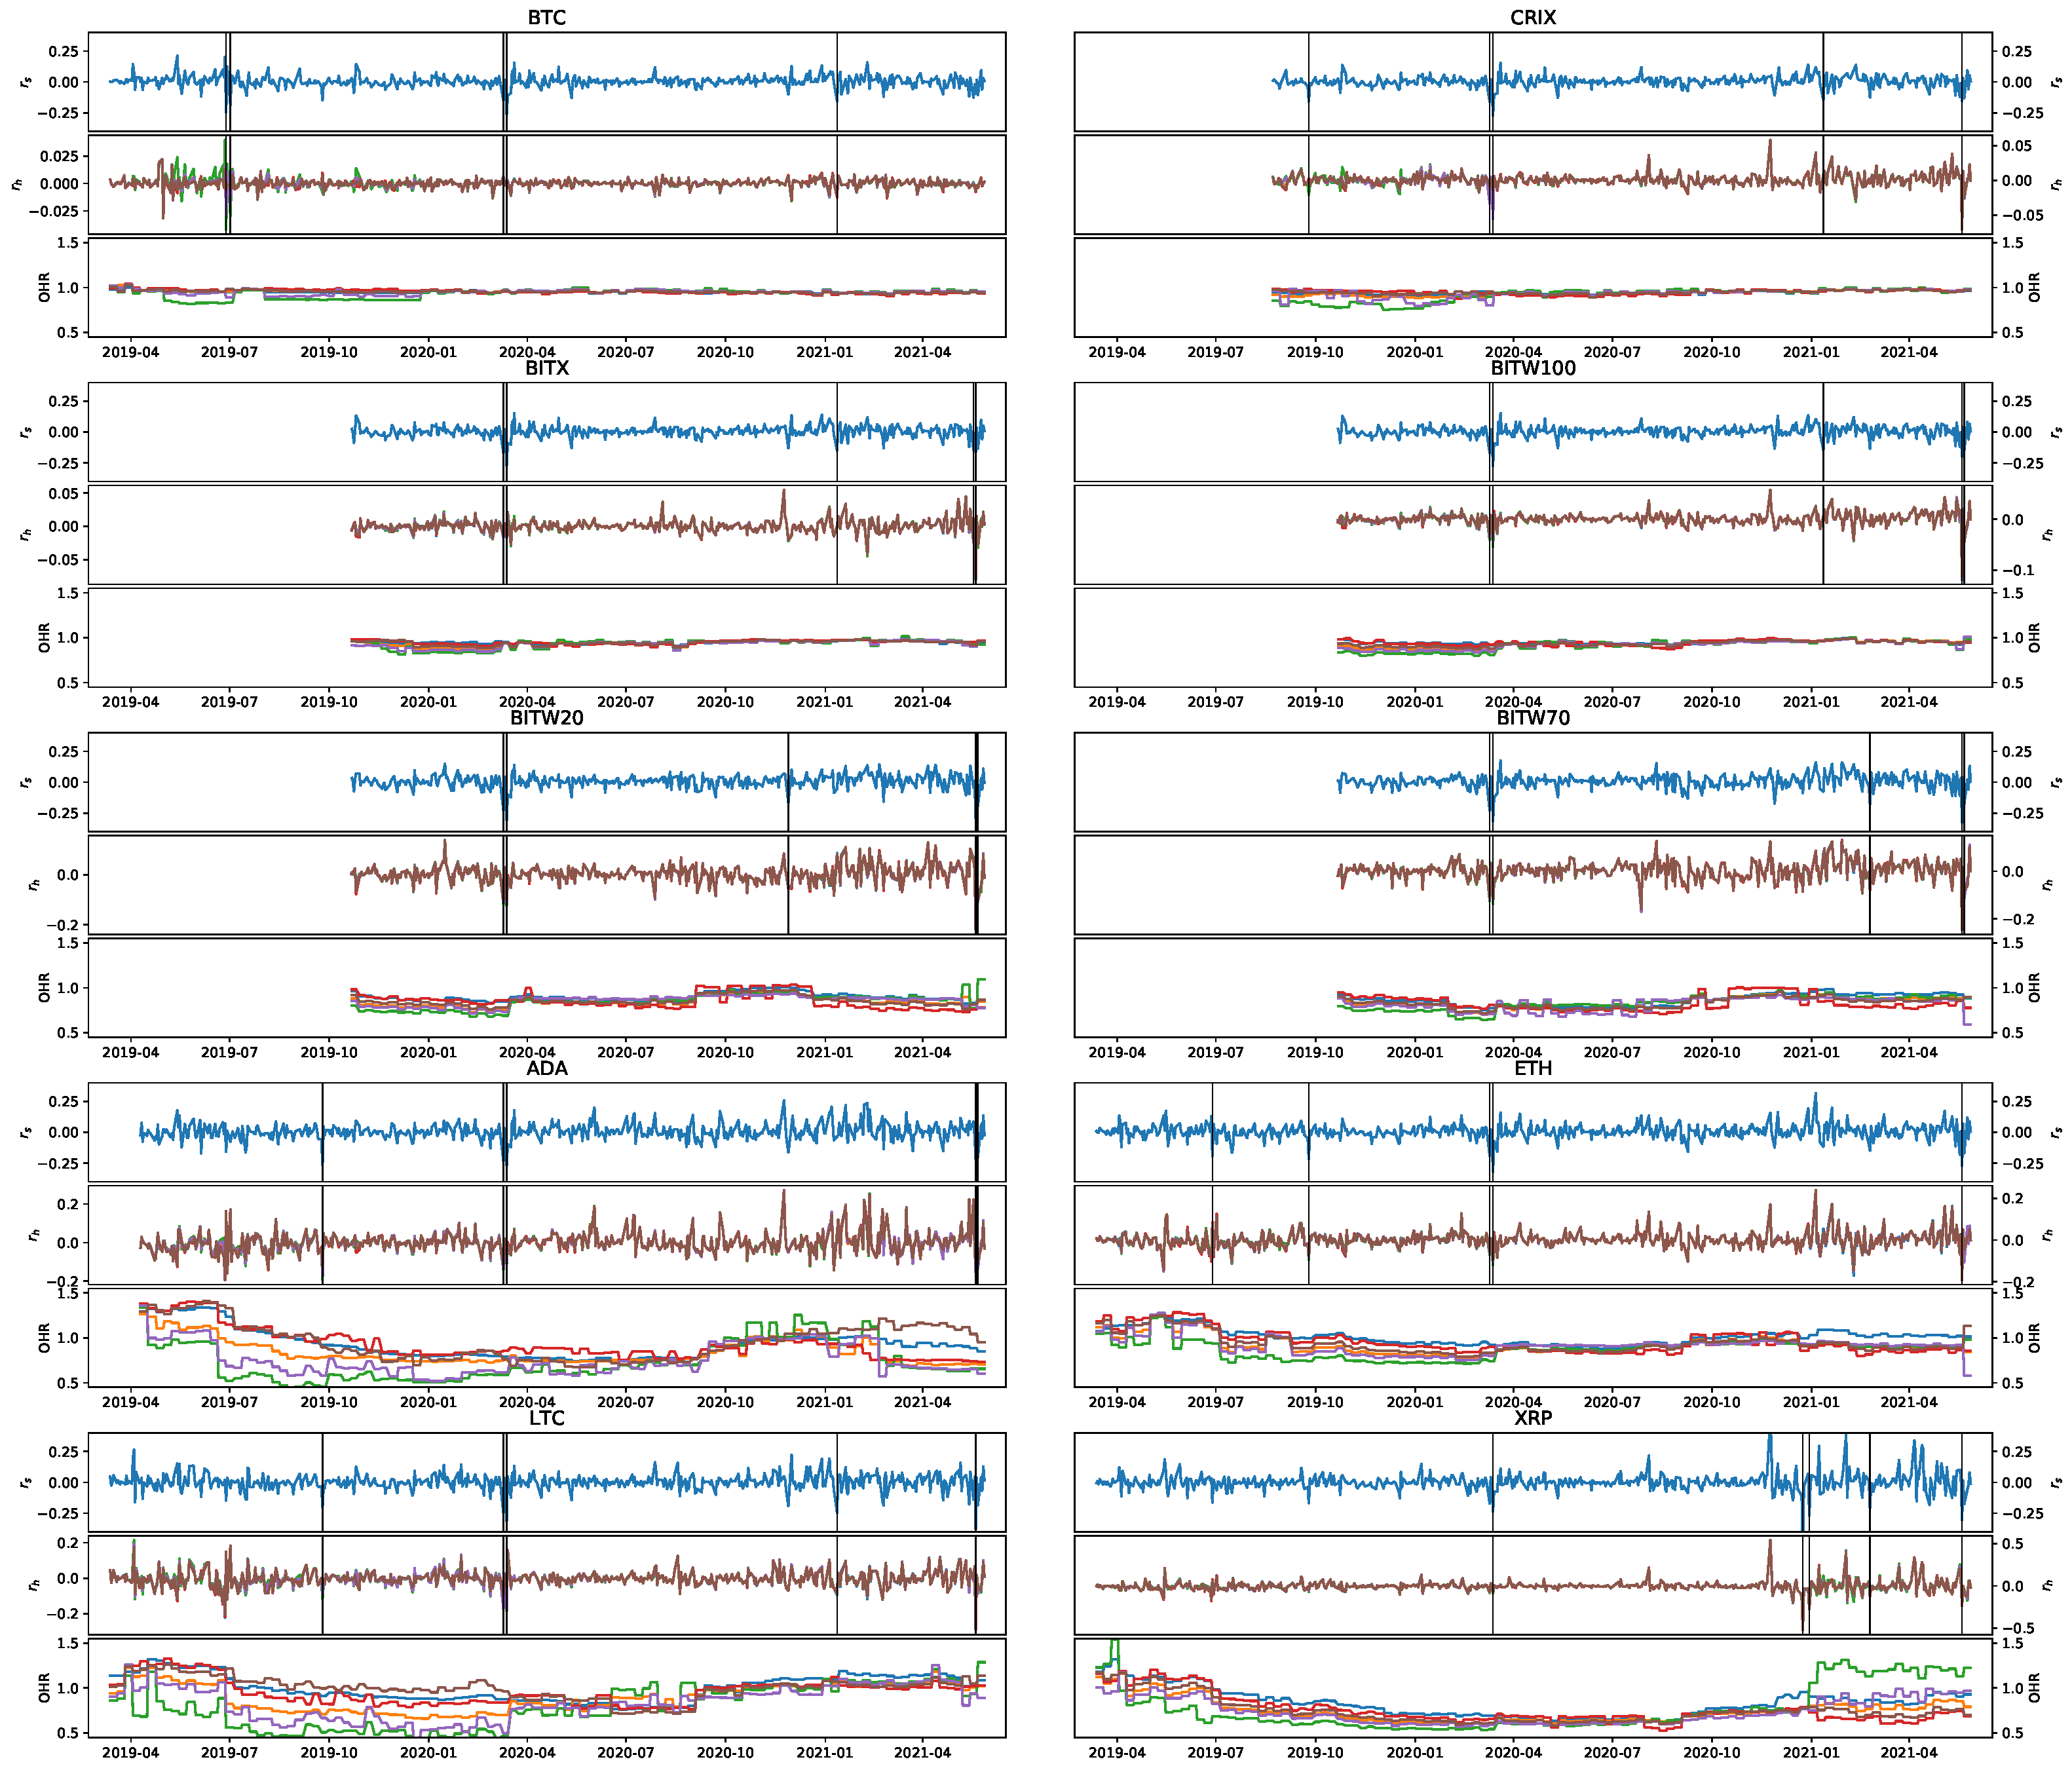
\includegraphics[width=0.9\paperwidth]{_pics/overview.pdf}
    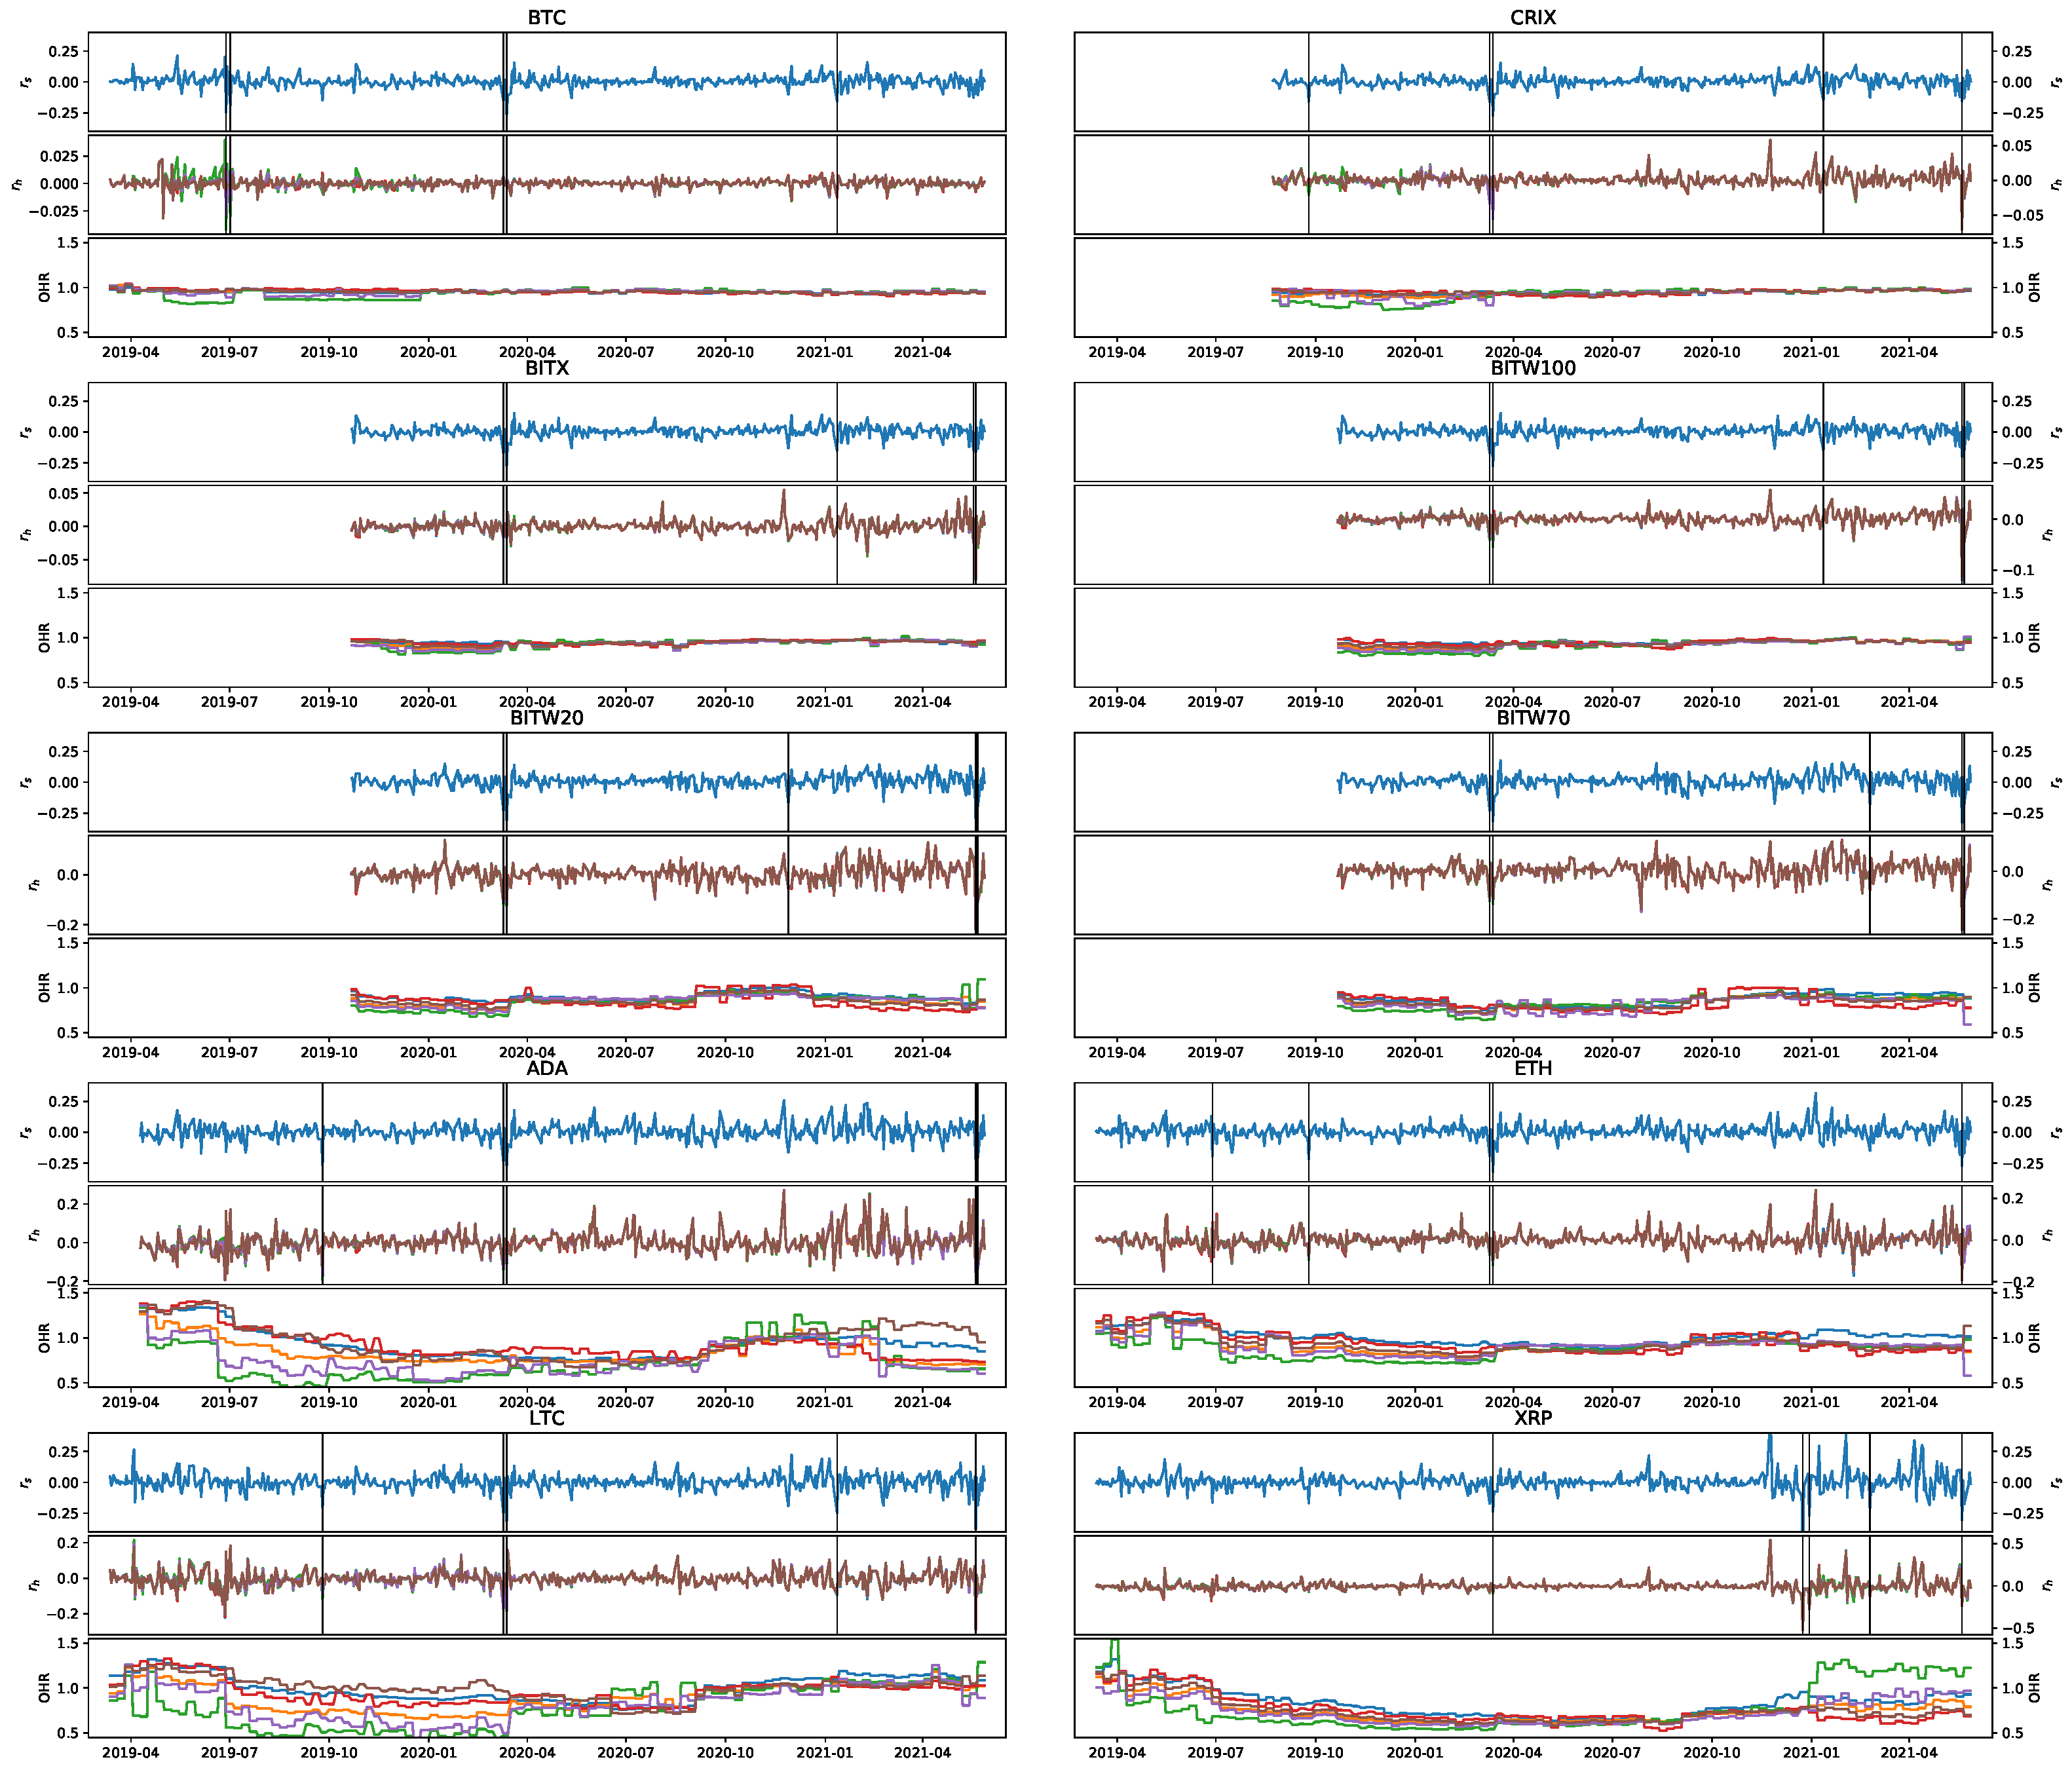
\includegraphics[width=\textwidth]{_pics/overview.pdf}
  \caption{An overview of out-of-sample hedged portfolios.
            For each panel, the line plot on the top is the daily log returns of the spot;
            line plot in the middle is the daily log returns of hedged portfolio with different risk reduction objectives;
            line plot at the bottom is the OHR of different risk reduction objectives. The coloring of risk reduction objectives is as follows:
                                      \textcolor{plt1}{blue line} for variance,
                                      \textcolor{plt2}{orange line} for ES 95\%,
                                      \textcolor{plt3}{green line} for ES 99\%,
                                      \textcolor{plt4}{red line} for VaR 95\%,
                                      \textcolor{plt5}{purple line} for VaR 99\%, and
                                      \textcolor{plt6}{brown line} for ERM $k=10$.
            The vertical black lines in the top and middle line plots indicate the dates when the five smallest returns occur in the spot return.
            Most of the time the portfolio returns of different risk minimisation objectives overlap wth each other.
            We can see that those BTC-involved spots, i.e. BTC, CRIX, BITX, and BITW100,  are well hedged by the BTCF as the magnitude of the hedged portfolio returns are greatly reduced,
            as well as the five extreme losses of the spots are well managed.
            One exception is the BTC-BTCF portfolio that minimize ES 99\% (first panel green line in middle plot), which fluctuate greatly from Jun 2019 to Aug 2019.
            In that period of time, the portfolio OHR is lower than its counterparts.
            Hedges of spots that are not BTC related are less promising.
            The effectiveness of a hedge is discussed in section \ref{sec: HE results}.
  \href{http://www.quantlet.com/}{\includegraphics[height=\baselineskip]{_pics/qletlogo_tr.png}} }
\label{fig:overview}
\end{figure}

In addition to the time series plots,
we inspect the performance of copula in hedging by the mean square error and lowersemi variance.
Mean square error is the distance between a perfect hedge and the hedged portfolio returns $\operatorname{MSE}=\frac{1}{n}\sum_{i=1}^n(r^h_i)^2$.
Lower semi variance is $\operatorname{LSV}=\frac{1}{n}\sum_{i=1}^n\{\operatorname{E}(r^h)r^h_i-\}^2$.
All results here are out-of-sample results obtained without the copula selection step in order to compare the performances across copulae.  \medskip

\begin{figure}[ht]
    \centering
    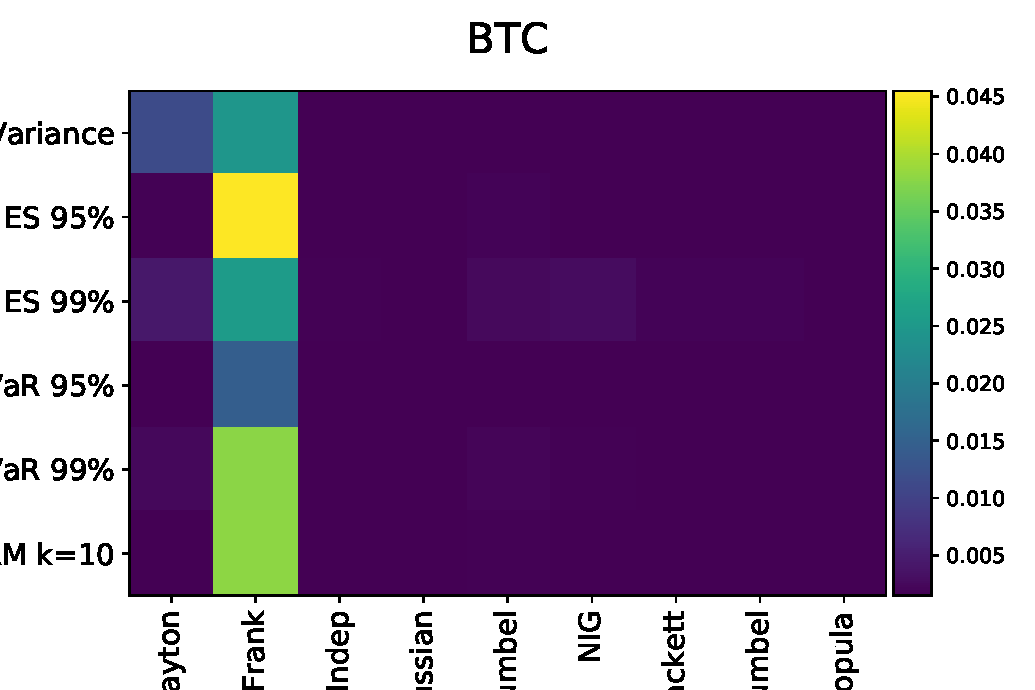
\includegraphics[width=\textwidth]{_pics/MSE_BTC.pdf}
  \caption{Mean square errors of BTC-BTCF portfolios constructed with different copula and risk minimization objectives.
    The Frank copula is inferior in the BTC-involved portfolios.
    \href{http://www.quantlet.com/}{\includegraphics[height=\baselineskip]{_pics/qletlogo_tr.png}} }
\label{fig:MSE_BTC}
\end{figure}

\begin{figure}[ht]
    \centering
    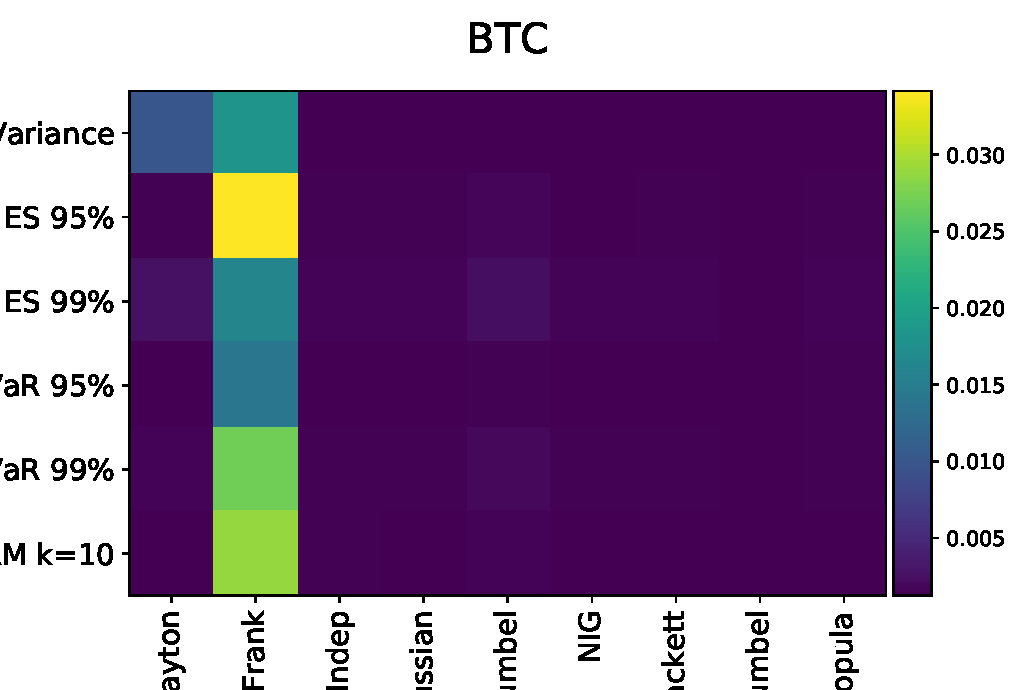
\includegraphics[width=\textwidth]{_pics/semiLowerVariance_BTC.pdf}
  \caption{Lower semivariance of BTC-BTCF portfolios constructed with different copula and risk minimization objectives.
  The Frank copula is obviously inferior.
  \href{http://www.quantlet.com/}{\includegraphics[height=\baselineskip]{_pics/qletlogo_tr.png}} }
\label{fig:SLV_BTC}
\end{figure}

\begin{figure}[ht]
    \centering
    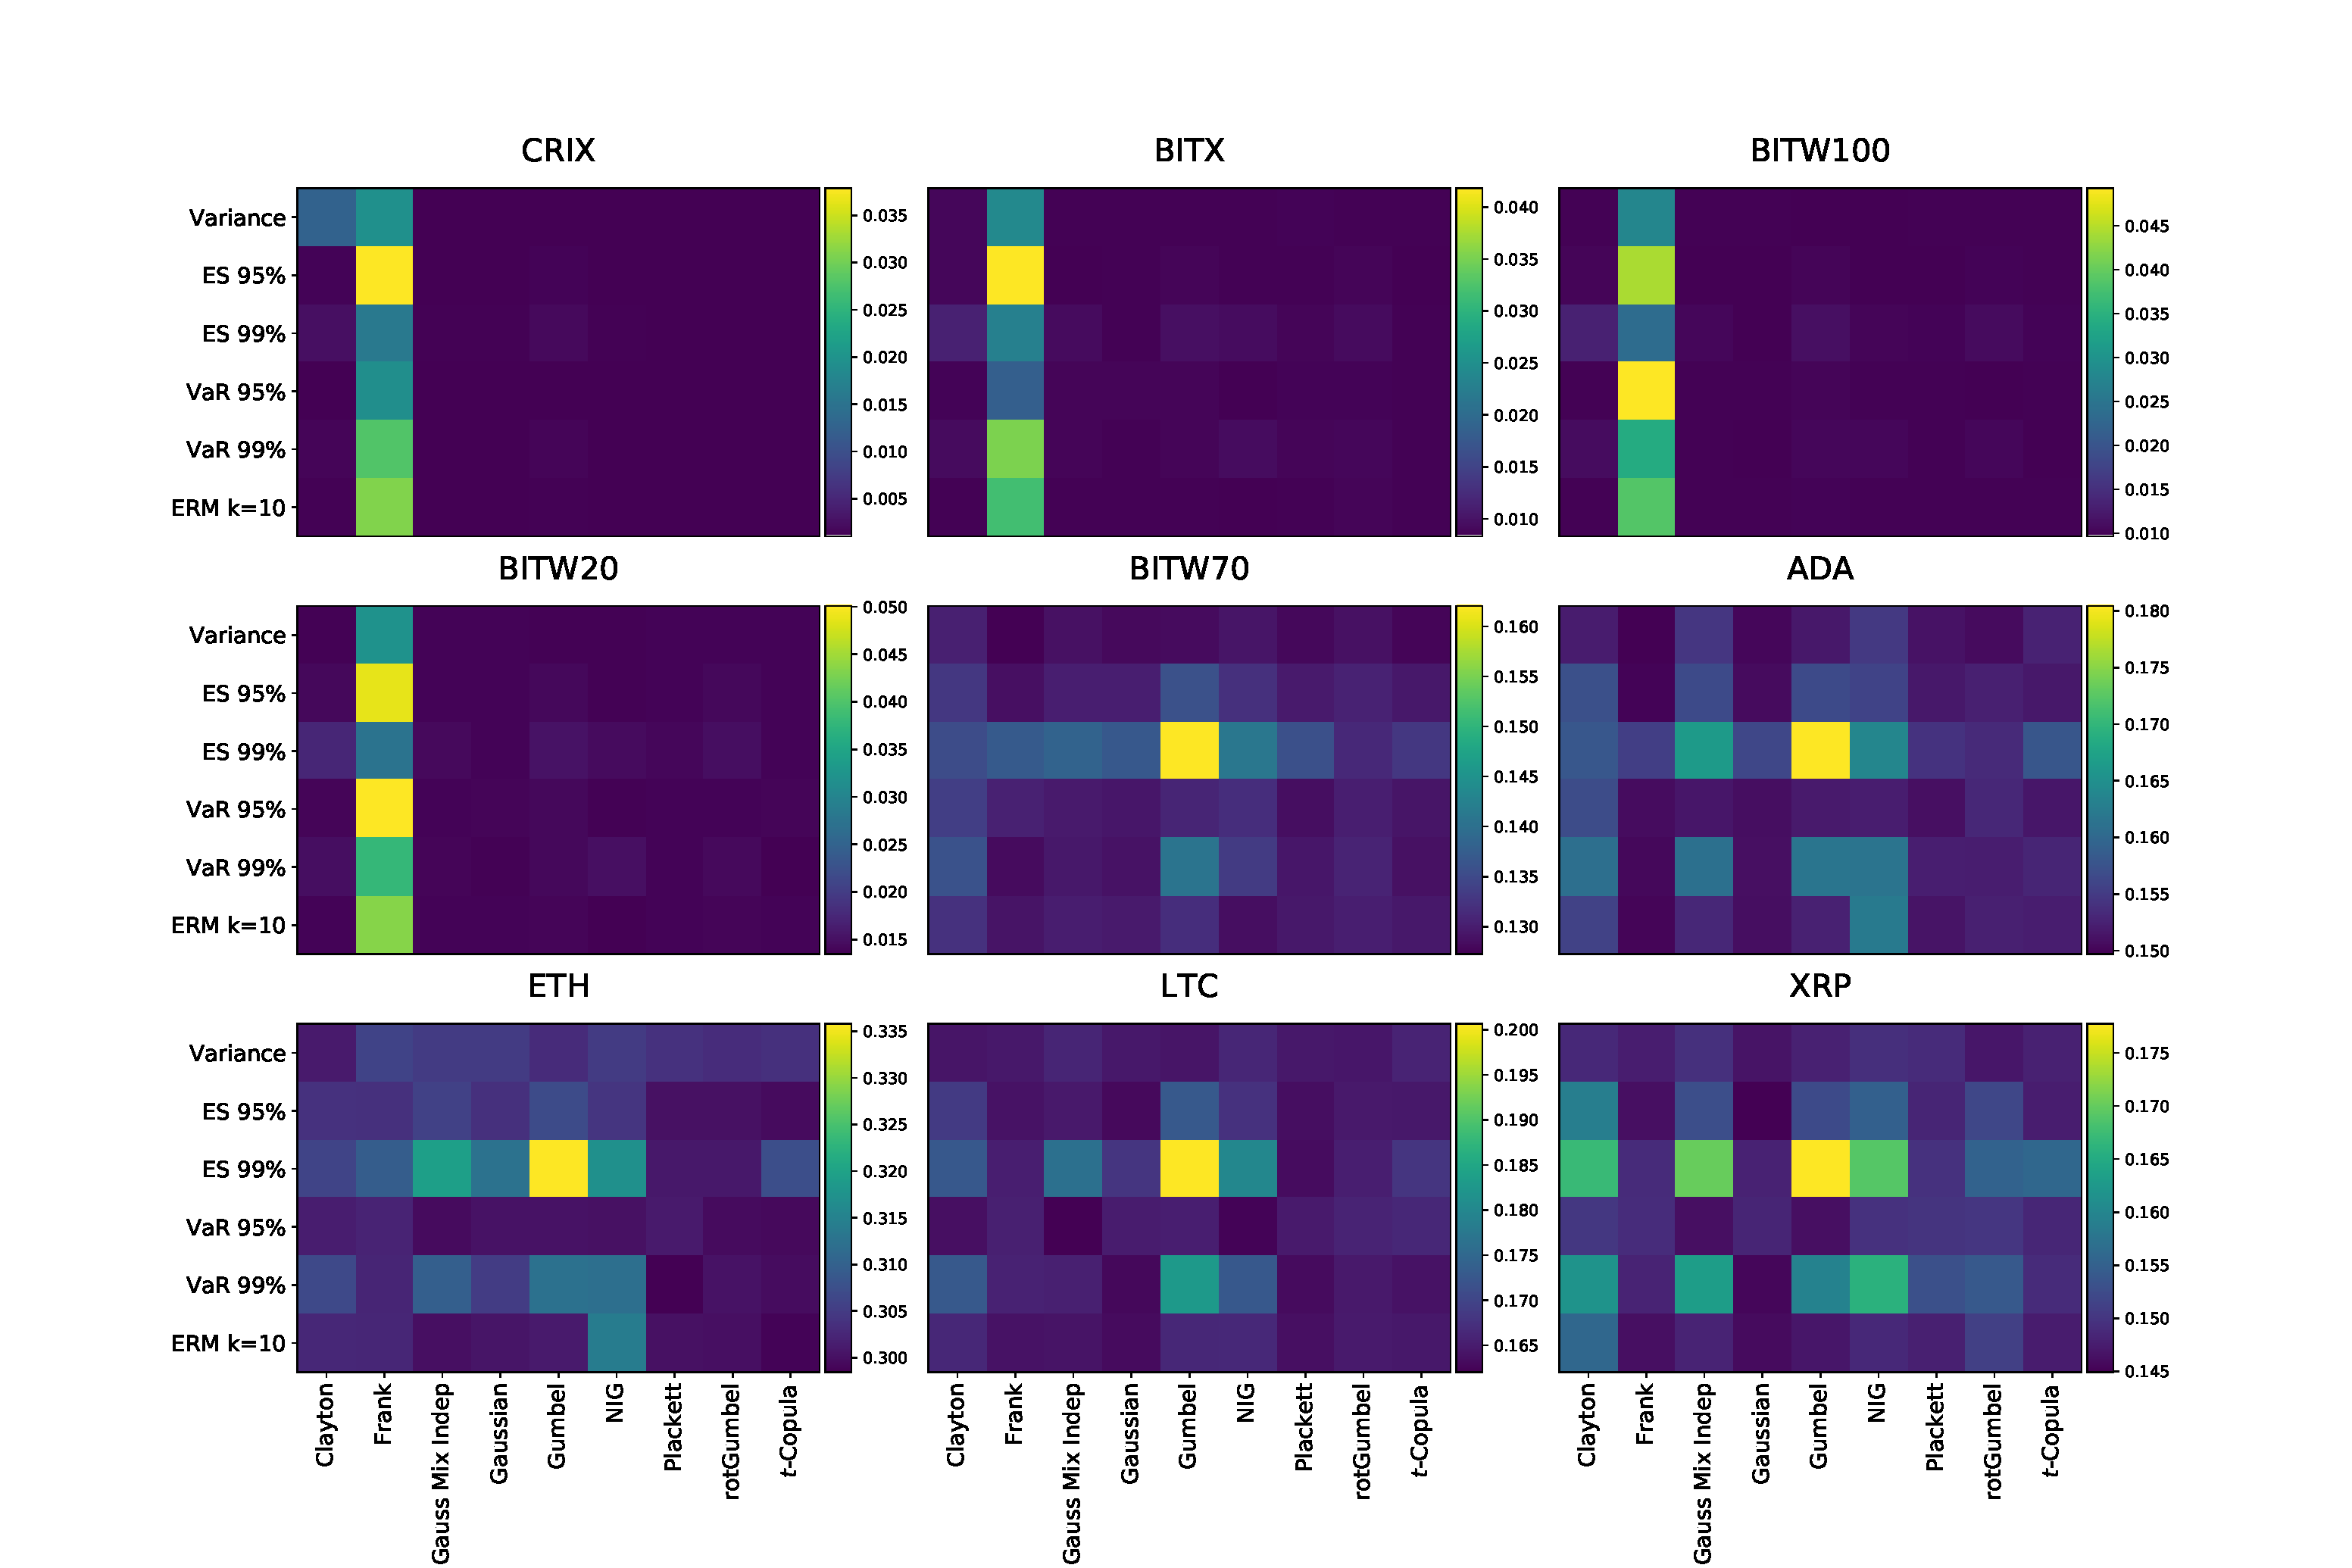
\includegraphics[width=\textwidth]{_pics/MSE_other.pdf}
  \caption{Mean square errors of portfolios constructed with different copula and risk minimization objectives.
  \href{http://www.quantlet.com/}{\includegraphics[height=\baselineskip]{_pics/qletlogo_tr.png}} }
\label{fig:MSE_other}
\end{figure}

\begin{figure}[ht]
    \centering
    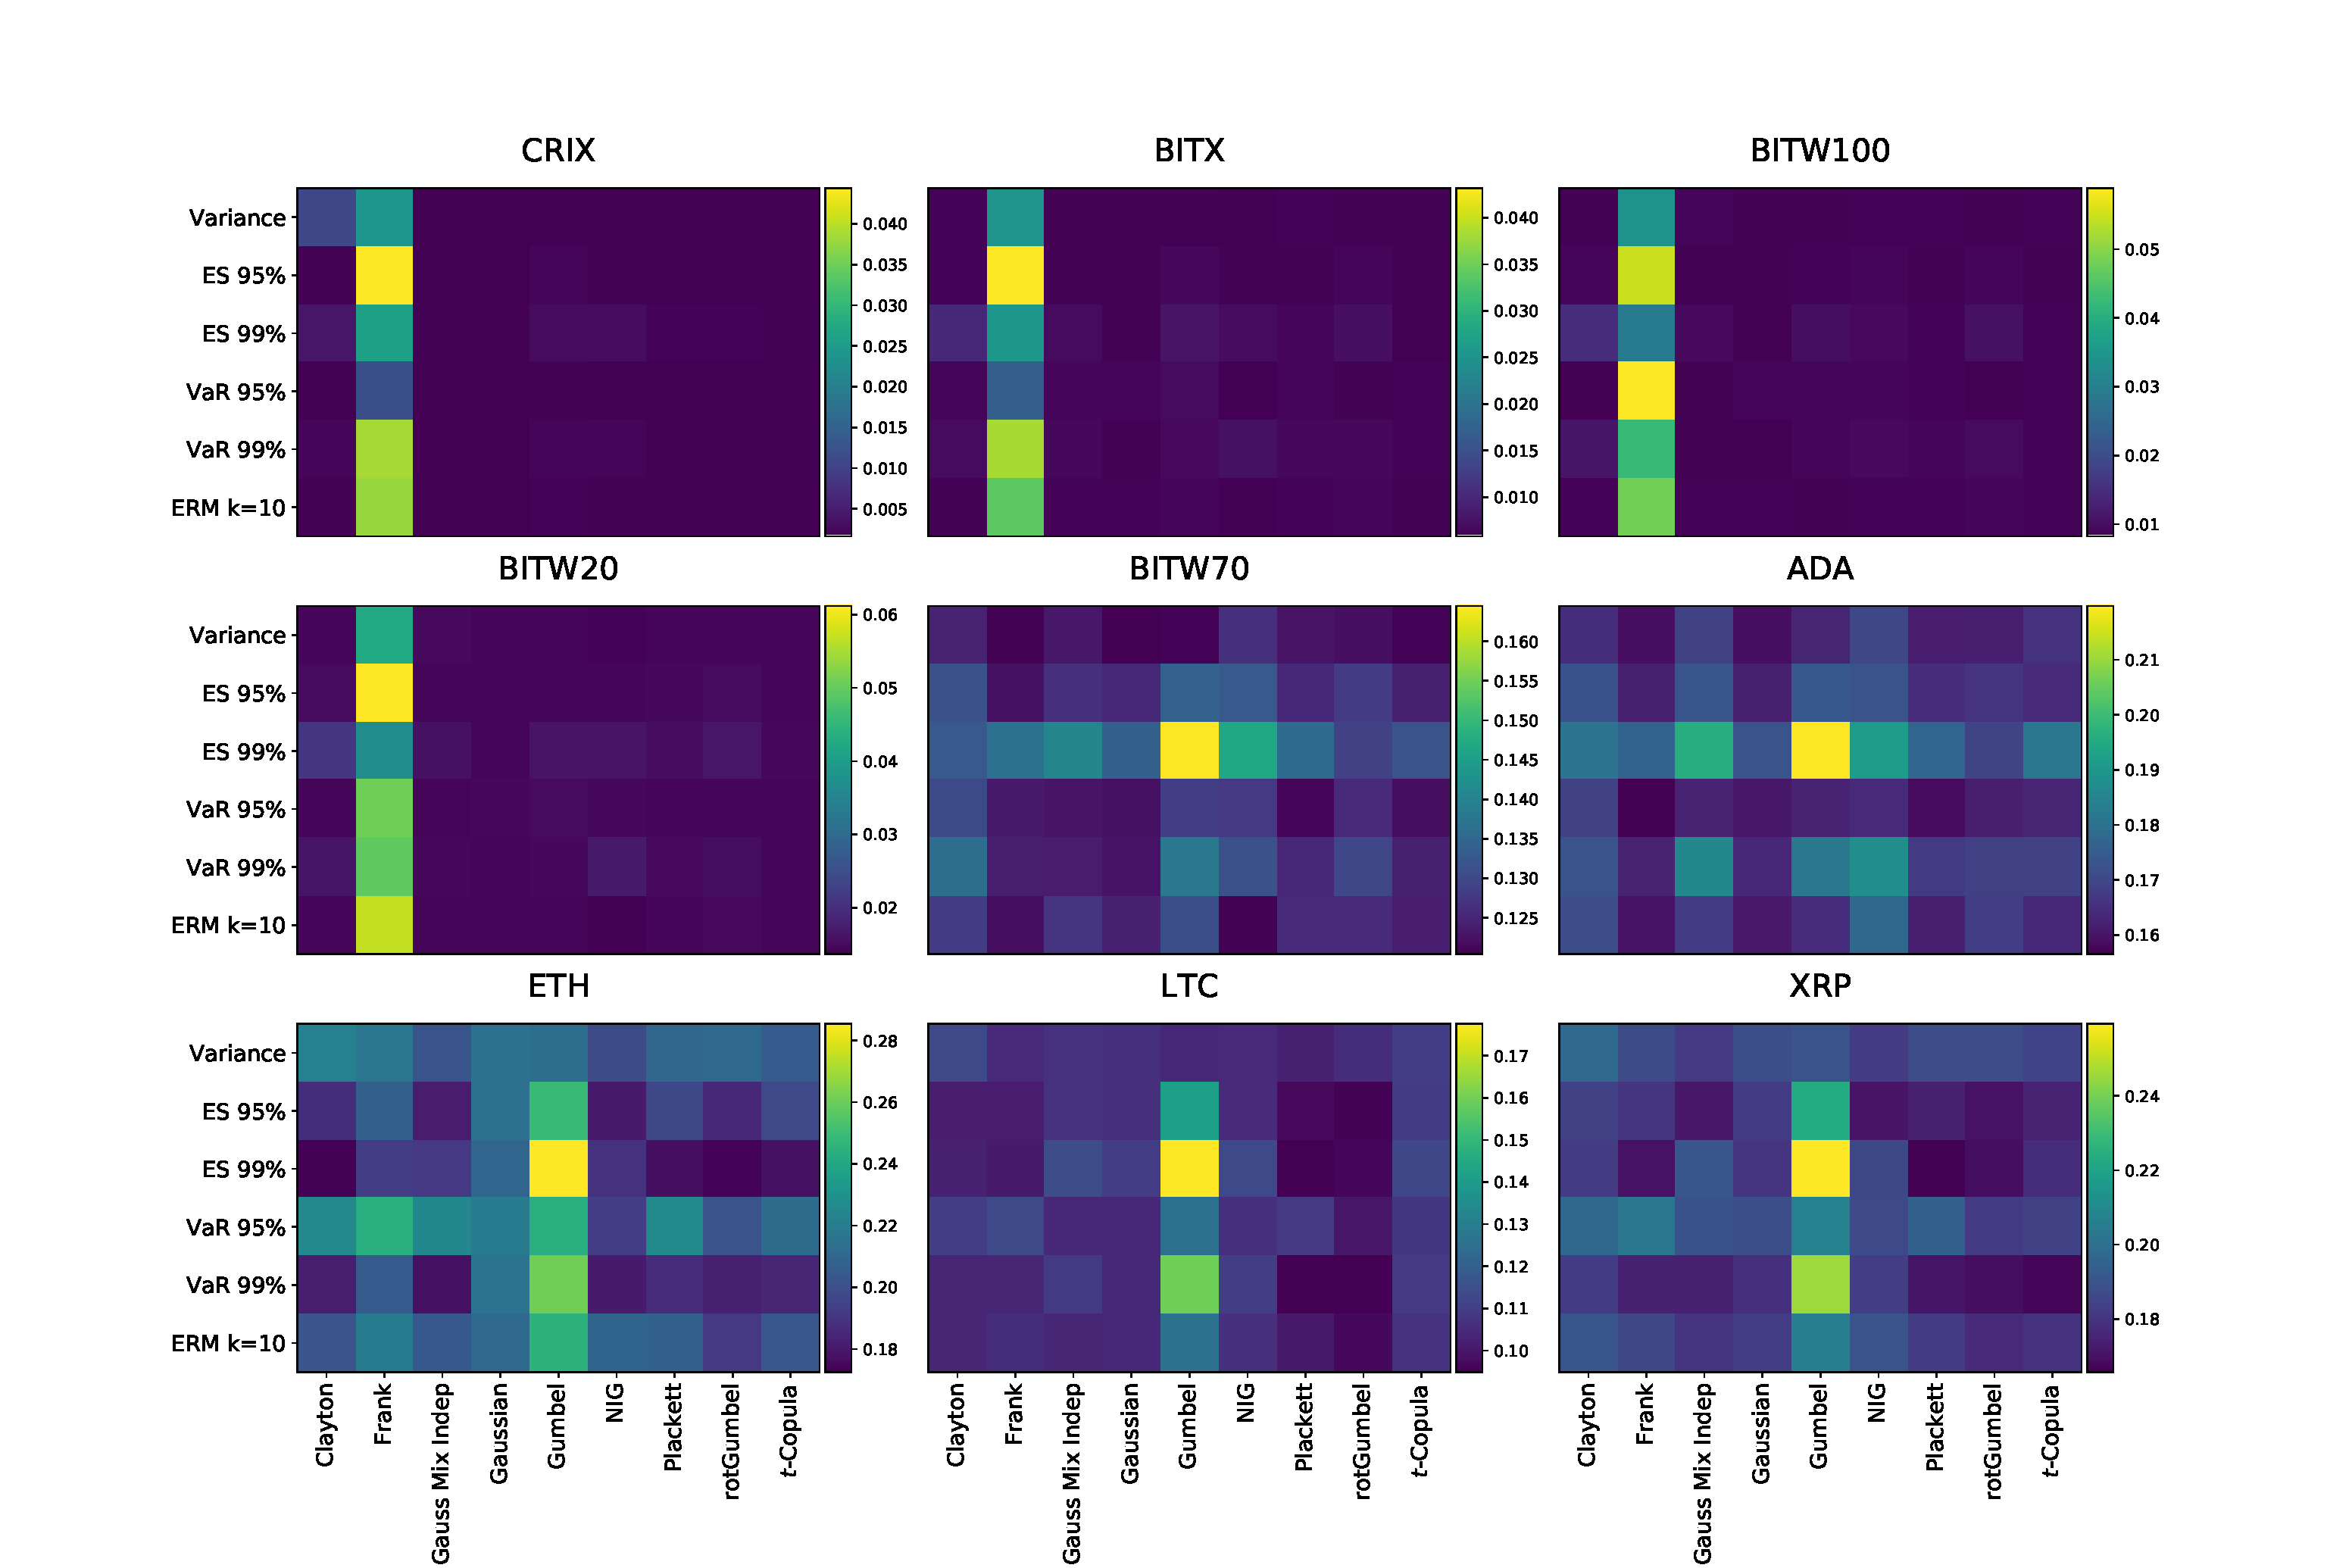
\includegraphics[width=\textwidth]{_pics/semiLowerVariance_other.pdf}
  \caption{Lower semivariance of portfolios constructed with different copula and risk minimization objectives.
  \href{http://www.quantlet.com/}{\includegraphics[height=\baselineskip]{_pics/qletlogo_tr.png}} }
\label{fig:SLV_other}
\end{figure}


Figure \ref{fig:MSE_BTC} and \ref{fig:SLV_BTC} are the mean square error and lower semivariance of BTC-BTCF, we can see the Frank copula is the worst performing copula:
the resulting hedged portfolio returns is far away from a perfect hedge.
In figure \ref{fig:MSE_other} and \ref{fig:SLV_other}, the phenomena of Frank copula being inferior to its counterparts can be observed from the results of the CRIX, BITX, BITW100, and BITW20-BTCF portfolios.
Interestingly, the spot in those portfolios usually have a strong dependency to the BTCF.
In contrast, the inferiority of the Frank copula is less prominent in the BITW70, ADA, ETH, LTC and XRP-BTCF portfolios.
We suspect that the Frank copula is not a choice to model assets with strong dependency.  \medskip

We can also observe from figure \ref{fig:MSE_other} and \ref{fig:SLV_other} that Gumbel copula is not performing as good as other copula in the ETH, LTC, and XRP-BTCF portfolios.
The reason is the Gumbel copula has only the upper tail dependence, while the ETH, LTC, and XRP exhibit lower tail dependency with BTCF.
We will discuss this in the following section. \medskip

Figure Xs also provide the information about the risk reduction objectives.
In general, portfolios that minimise variance, ES 95\%, VaR 95\%, and ERM are very similar in means square error and lower semi variance.
Contrarily, portfolios that minimise ES 99\% and VaR 99\% are have high mean square error and lower semi variance.
This may due to the fact that ES 99\% and VaR 99\% are easily affected extreme events in the training data. \medskip
%We will further discuss the issue in section X.  \medskip

\subsection{Copula Selection Results}\label{sec: copula results}
The copula selection result provides insight that help us understand the crypto market better, so
we illustrate the copula selection result in this section.
Decisions of the AIC procedure are summarised in table \ref{tab:copulasection}. \medskip

Overall, $t$-copula, rotated Gumbel (rotGumbel), and the NIG factor copula are the most frequently chosen copulae by the AIC procedure. \medskip

The $t$-copula is frequently chosen by AIC to model the dependency between the BTC and BTC involved indices, CRIX, BITX, BITW100, and the BTC future.
BTC and BTC involved indices exhibit strong tail dependence (both upper and lower tail) with BTCF.
We could interpret tail dependence much more of a tendency for one asset to be extreme when another is extreme and vice versa \citep{McNeil2015}.
In fact, the $t$ copula has been suggested in various empirical studies to model financial data, such as \cite{zeevi2002beyond} and \cite{breymann2003dependence}.
Those studies suggest $t$-copula is a better model over the Gaussian copula which financial data often seem to exhibit tail dependence. \medskip

On the other hand, the radially symmetric feature makes the $t$-copula not a good choice to model the other hedging pairs.
\cite{demarta2005t} describe the symmetry feature "strong", because if $(U_1, ..., U_d)$ is a vector distributed in $t$-copula,
then $(U_1, ..., U_d) \overset{\mathcal{L}}= (1-U_1, ..., 1-U_d)$.
This symmetry can be justified in the dependence structure between a futures and its underlying by the theory of futures pricing,
which suggests the price of a futures is a function of the underlying price \citep{hull2003options}.
However, there is no such relationship between a futures and an asset which is not the underlying, and so the radial symmetry becomes a drawback to model other hedging pairs e.g. ETH and BITX70.
Another drawback of the $t$-copula is the lack of flexibility to model off-diagonal region since Rho and nu jointly control the density of the off-diagonal region.
%The off-diagonal region (HF paper breymann2003dependence)
This is why sometimes the Gaussian Mix Independence (GMI) better model the dependence.  \medskip

Among the three popular copulae, rotGumbel copula shows its ability to model the dependency between ETH and BTCF,
94 out of 112 training sets are best fitted with the rotated Gumbel.
rotGumbel also performs well when modelling dependency between XRP, BITW20, BITW70, and the BTCF.
In particular, the whole time series of the two indices, BITW20 and BITW70, are best fitted solely with the rotated Gumbel copula.
The frequently chosen rotated Gumbel indicates the styled fact of financial data: prices tends to drop together.  \medskip
%  (ref) The reason for that

%The rotated Gumbel model the lower tail dependency very well, it has a lower quantile dependence controlled by its parameter

%BTC upper tail dependence BTC lower tail dependence (with fitted copula (t and rotGumbel) tail dependence)

%ETH upper tail dependence ETH lower tail dependence (with fitted copula (t and rotGumbel) tail dependence)

In fact, Clayton's AIC in many of the training sets is the second lowest, just higher than that of rotated Gumbel.
This is because the Clayton copula has the same ability to model the lower quantile dependence.
However, Clayton's radial like feature does not match the behaviour of the financial data. \medskip

It is worth to mention that although the NIG factor copula is penalised heavily due to its three parameters setup, it is frequently chosen to be the best copula to model the dependency between individual cryptos and the BTC future.
An extreme case would be ADA, only NIG factor is chosen in our dataset.
Another dependency structure being best described by the NIG factor copula is the pair of LTC-BTCF.
64 out of 112 training sets are best fitted by the NIG factor copula.
Indices like BITX and CRIX are sometimes best fitted with the NIG factor copula as well, accounting for modelling 12 and 27 training sets respectively.
The popularity of the NIG factor reflects the ability of the copula to model very complex dependency structure.
NIG factor copula is able to model the tail, radial asymmetry, and off diagonal behaviour.  \medskip %(ADA samples and fitted NIG samples)

Frank copula is generally not a good choice to model financial data just like what \cite{barbi2014copula} has reported.
Plackett is known for its dependence parameter can be written as the cross-product ratio \citep{joe1997multivariate}.
However, this feature does not bring the Plackett Copula advantage over other copulae to model the dependence structure between cryptos and BTCF. \medskip

\begin{table}[t!]
 \ra{1.1}
    {\begin{tabularx}{\textwidth}{lYYYYY} \toprule
         Copula/Asset & $t$ & Plackett & GMI & rotGumbel & NIG \\ \midrule
     \multicolumn{6}{l}{Individual Cryptos}                                                                                 \\
        \ \ \ BTC          & 73         & 4                 & 2                        & 1                  & 31                  \\
        \ \ \ ETH          & 3          & 6                 & 8                        & 94                 & 1                   \\
        \ \ \ ADA          & 0          & 0                 & 0                        & 0                  & 112                 \\
        \ \ \ LTC          & 13         & 0                 & 3                        & 32                 & 64                  \\
        \ \ \ XRP          & 0          & 31                & 3                        & 78                 & 0                   \\
   \multicolumn{6}{l}{Crypto Indices with BTC Constituent}                                                                  \\
        \ \ \ BITX         & 39         & 0                 & 14                       & 16                 & 12                  \\
        \ \ \ CRIX         & 47         & 0                 & 11                       & 3                  & 27                  \\
        \ \ \ BITW100      & 42         & 0                 & 8                        & 29                 & 2                   \\
    \multicolumn{6}{l}{Crypto Indices without BTC Constituent}                                                              \\
        \ \ \ BITW20       & 0          & 0                 & 0                        & 78                 & 3                   \\
        \ \ \ BITW70       & 0          & 0                 & 0                        & 80                 & 1                   \\
    \bottomrule
    \end{tabularx}
        \caption{Copula Selection Results. }









\label{tab:copulasection}}
\end{table}

\subsection{OHRs and Returns of Hedged Portfolios}\label{sec:results overview}
We present an overview of the OHR and hedged portfolios log returns results in this section.
Overall, the performance of the hedge largely depend on the spot assets, while the choice of risk minimisation objective does not affect much of the log return of hedge ratio.
We present the summary statistics of the hedged portfolios returns in table \ref{tab:ERMrh} that aimed at minimising ERM $k=10$. \medskip
%Detail summary statistics of the hedged portfolios returns are documented in the appendix from table 1 to table 10. \medskip

\begin{table}[t!]
\begin{table}[!] \centering \resizebox{\textwidth}{!}{%
\begin{tabular}{lrrrrrrr} \toprule
         {} &    Mean \% &     Std \% &      Skew &       Kurt &         MD \% &     MD date & ERM k=10 \\
\midrule
     \multicolumn{7}{l}{Individual Cryptos}                                                                                 \\
\ \ \ BTC     &  0.0223 &  0.3221 & -1.0008 &   3.4153 &  -1.5242 &  2020-11-30 &    0.0057 \\
\ \ \ ETH     &  0.3117 &  3.8679 &  1.0345 &   7.5751 & -18.8729 &  2021-05-19 &    0.0491 \\
\ \ \ ADA     &  0.5722 &  5.3590 &  1.4203 &   4.6970 & -14.3885 &  2021-01-08 &    0.0700 \\
\ \ \ LTC     & -0.0512 &  3.8812 & -0.2929 &   7.7022 & -28.0879 &  2021-05-19 &    0.0616 \\
\ \ \ XRP     &  0.0155 &  7.1579 &  1.1244 &  19.8583 & -52.5689 &  2020-12-23 &    0.0787 \\
   \multicolumn{7}{l}{Crypto Indices with BTC Constituent}                                                                  \\
\ \ \ BITX    &  0.0590 &  1.0078 & -0.4427 &  13.0839 &  -7.8581 &  2021-05-19 &    0.0127 \\
\ \ \ CRIX    &  0.0840 &  0.9087 &  0.0488 &  14.5501 &  -7.0530 &  2021-05-19 &    0.0100 \\
\ \ \ BITW100 &  0.0853 &  1.2032 & -1.6522 &  20.5562 & -11.1846 &  2021-05-19 &    0.0153 \\
    \multicolumn{7}{l}{Crypto Indices without BTC Constituent}                                                              \\
\ \ \ BITW20  &  0.2564 &  3.6009 & -0.3446 &   4.2152 & -21.5920 &  2021-05-19 &    0.0503 \\
\ \ \ BITW70  &  0.2818 &  3.9074 & -0.6952 &   4.8745 & -24.5250 &  2021-05-19 &    0.0557 \\
\bottomrule
\end{tabular}}
\caption{Summary statistics of out-of-sample daily returns of hedged portfolios that minimize ERM $k=10$.}
\label{tab:ERM_rh}

\end{table}

\caption{Statistics of daily log returns  of hedged portfolios aimed at minimizing ERM $k=10$.}
\label{tab:ERMrh}
\end{table}

We can see from table \ref{tab:ERMrh} that the summary statistics of hedged portfolio returns differ.
As expected, the BTC-involved portfolios, i.e. portfolios with BTC, CRIX, BITX, and BITW100 as spot, have a relatively small
standard deviations (std) and maximum drawdowns (MD).
However, the kurtosis (kurt) of the portfolio returns are higher than the other portfolios except XRP.
This result suggests that the variance of the BTC-involved spots are well hedged but not the jump risk (extreme events).
In fact, extreme events are hard to model and predict, even the BTC-BTCF portfolio cannot escape from this.
Nonetheless, the skewness (skew) are close to zero. \medskip

Portfolios with spot of crypto indices that are not BTC-involved, i.e. BITW20 and BITW70, have relatively lower std and MD than portfolio with individual cryptos as spot.
This indicates the overall market is indeed follow the BTC or the BTCF's development, but individual cryptos can have their own price movement just as discuss in the last section. \medskip

Next, we illustrate the OHR time series of the BTC-BTCF and other hedge portfolios in figure \ref{fig:BTCOHR} and \ref{fig:OHR-timeseries} respectively.
The two most fluctuating OHR time series are generated by minimising ES 99\% and VaR 99\%.
ES 99\% and VaR 99\% are calculated based on a small fraction of data from the left tail of portfolio return,
so the resulting OHR time series are relatively sensitive to extremes in the training data.
The other OHR time series do not deviate from each other a lot. \medskip

\begin{figure}[t]
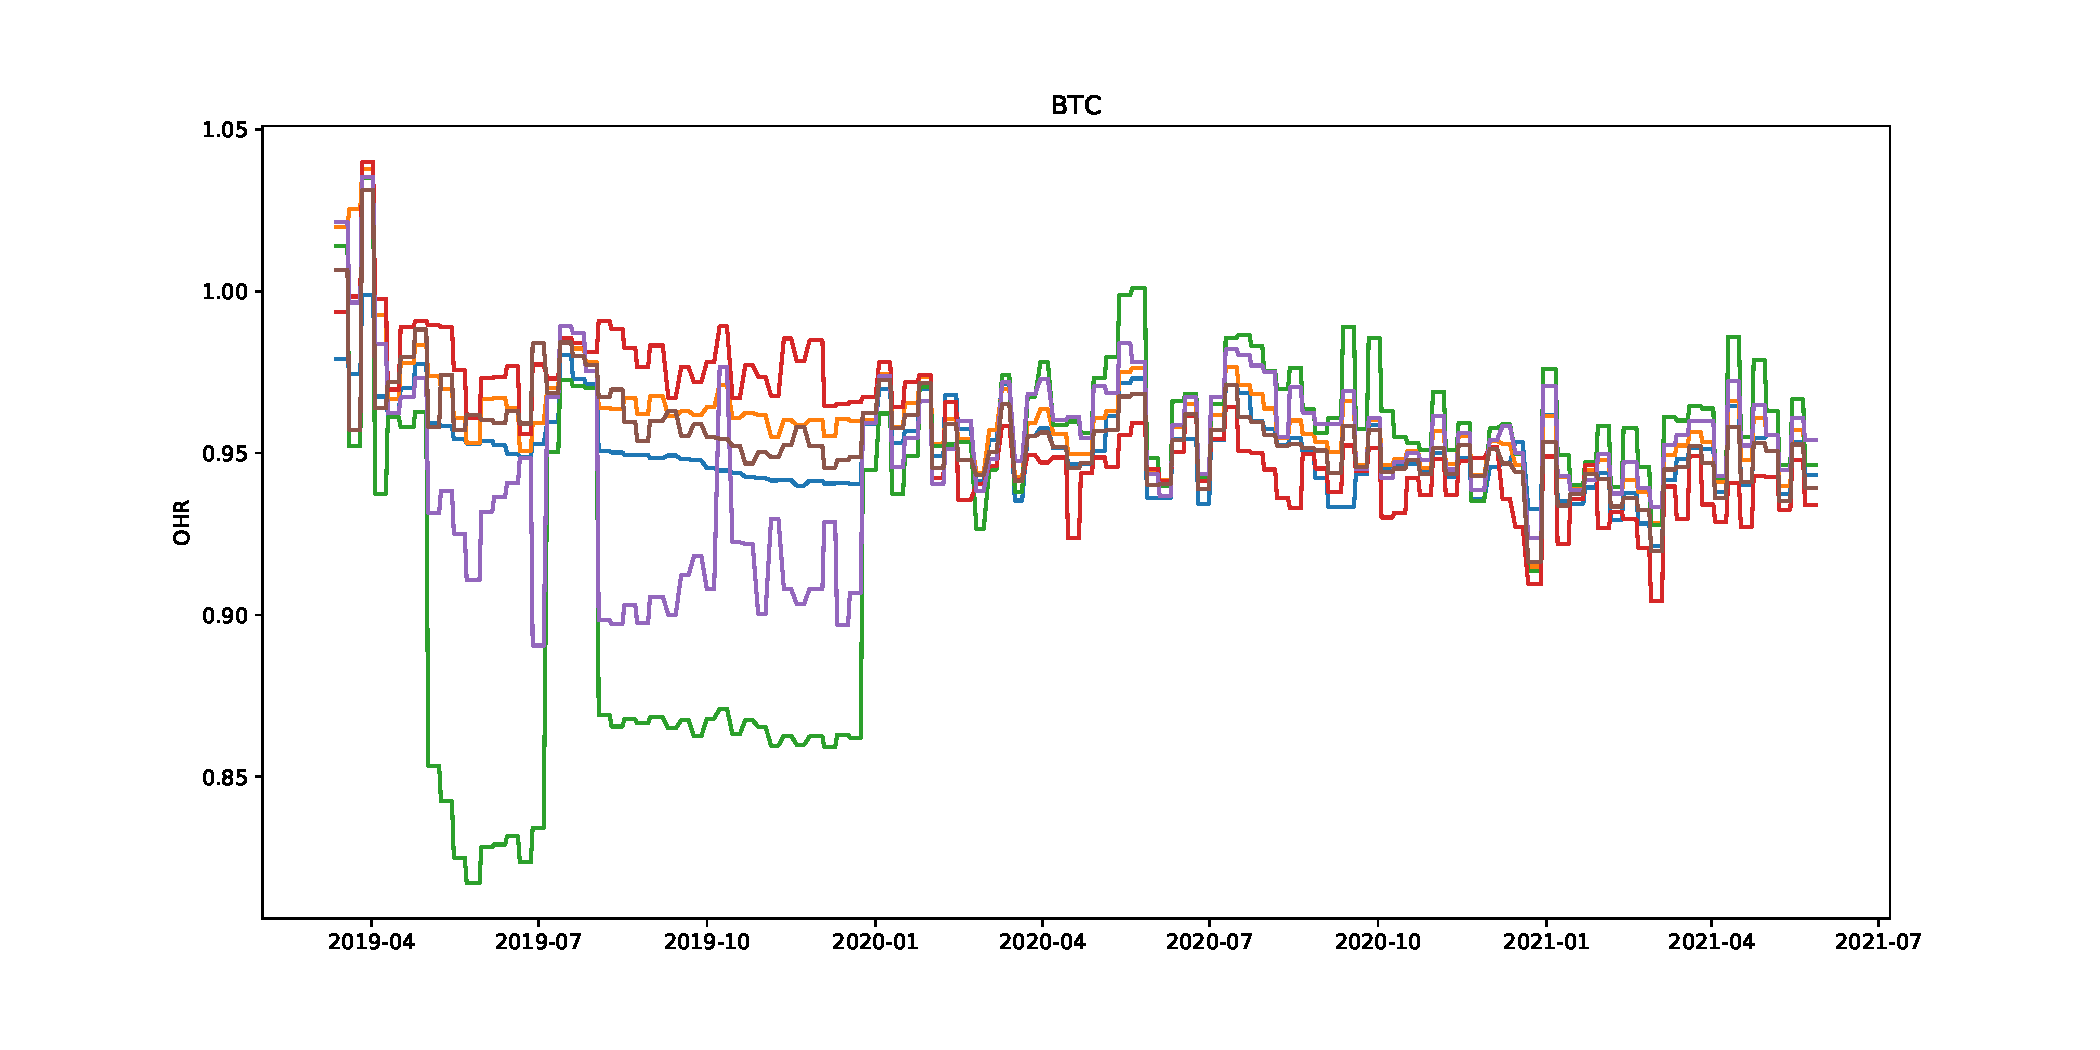
\includegraphics[width=\textwidth]{_pics/BTC_OHR.pdf}
  \caption{OHR of BTC-BTCF portfolio with different risk minimizing objectives. The \textcolor{plt1}{blue line} is OHR minimizing variance,
                                      \textcolor{plt2}{orange line} is that of ES 95\%,
                                      \textcolor{plt3}{green line} is that of ES 99\%,
                                      \textcolor{plt4}{red line} is that of VaR 95\%,
                                      \textcolor{plt5}{purple line} is that of VaR 99\%, and
                                      \textcolor{plt6}{brown line} is that of ERM $k=10$.
  \href{http://www.quantlet.com/}{\includegraphics[height=\baselineskip]{_pics/qletlogo_tr.png}} }
\label{fig:BTCOHR}
\end{figure}

In figure \ref{fig:OHR-timeseries}, we can observe a large range of OHR in other hedge portfolios.
For BTC-involved indices, the OHRs are ranging from 0.75 to 1.05, slightly wider than range of BTC-BTCF's OHR. \medskip

Again, we present the OHR time series generated by minimising ES 99\% and VaR 99\% are more fluctuating in different hedge portfolios.
Furthermore, we can see more clearly in figure \ref{fig:OHR-timeseries} that OHR minimising ES 99\% are more extreme. \medskip

\subsection{Hedging Effectiveness Results}\label{sec: HE results}
In this section, we analyse the out-of-sample hedging effectiveness (HE) of BTCF as hedging.
HE is defined as $$\text{HE} = 1-\frac{\rho_h}{\rho_s},$$
a measure of the percentage reduction of portfolio risk attribute, in our case the spot $\rho_s$,
to hedged portfolio risk attribute $\rho_h$.
A higher HE indicates a higher hedging effectiveness and larger risk reduction. \medskip

The HE above is a generalisation of Ederington measure of hedging performance, where we,
in addition to variance, include other risk measures: Expected Shortfall 5\% and 1\% (ES5 and ES1), Value-at-Risk 5\% and 1\% (VaR5 and VaR1), and ERM.
In particular, ES5 is recommended by the Basel Committee on Banking Supervision (BCBS) to replace VaR as a quantitative risk metrics system.
The proposed reform aimed at enhancing the risk metric system's ability to capture tail risk. \medskip
%Discussions of the issue can be found in literatures.
%
We obtain a time series of out-of-sample $r^h$ of each hedging pair and each risk reduction objective by concatenating the out-of-sample results.
Then, we apply stationary block bootstrapping (SB) to the time series introduced by \cite{Politis1994} in our analysis in order to preserve the temporal structure of the data while sampling.
The SB procedure is as follow.
Assume a time series with $N$ observations $\{X_t\}_{t \in [1,N]}$ is a strong stationary, weakly dependence time series of interest,
we form blocks of samples $B = \{X_i, ..., X_{i+j-1}\}$.
Index $i$ is a random variable uniformly distributed over $[1,2,...,N]$ and $j$ is geometric distributed random variable with parameter .
The block index $i$ and block length $j$ are independent.
For any index $k$ which is greater than $N$, the sample $X_k$ is defined to be $X_{k(\mod N)}$.
For each block, we calculate the hedging effectiveness with different risk measures mentioned above.
We choose $p=0.005$, implying the expected block length is 200.
100 blocks are drawn for each risk minimising objective and spot. \medskip

From figure \ref{fig:HEboxplot}, we report, as expected, the BTC involving spots, the BTC, CRIX, BITX and BITW100, are well hedged by the BTCF.
Surprisingly, the performances are consistent across different risk reduction objectives and different HE evaluation.
The median HE to BTC generated by various risk reduction objectives is ranging from 89.45\% to 99.31\%, median HE to CRIX is ranging from 81.13\% to 95.22\%,
median HE to BITX is ranging from 79.06\% to 94.84\%, median HE to BITW100 Is ranging from 71.07\% to 92.98\%. \medskip

The HE of BTCF to other cryptos and indices are substantially lower than to the BTC involving spots, but the consistency the performances across different risk reduction objectives and HE evaluation remains.
The median HE to BITW20 generated by various risk reduction objectives is ranging from 24.67\% to 47.02\%, median HE to BITW70 is ranging from 23.61\% to 49.30\%,
median HE to ADA is ranging from 9.01\% to 29.30\%, median HE to ETH Is ranging from 30.07\% to 36.18\%, median HE to LTC Is ranging from 37.74\% to 51.30\%,
median HE to XRP Is ranging from 0.46\% to 30.89\%.
\begin{figure}[h]
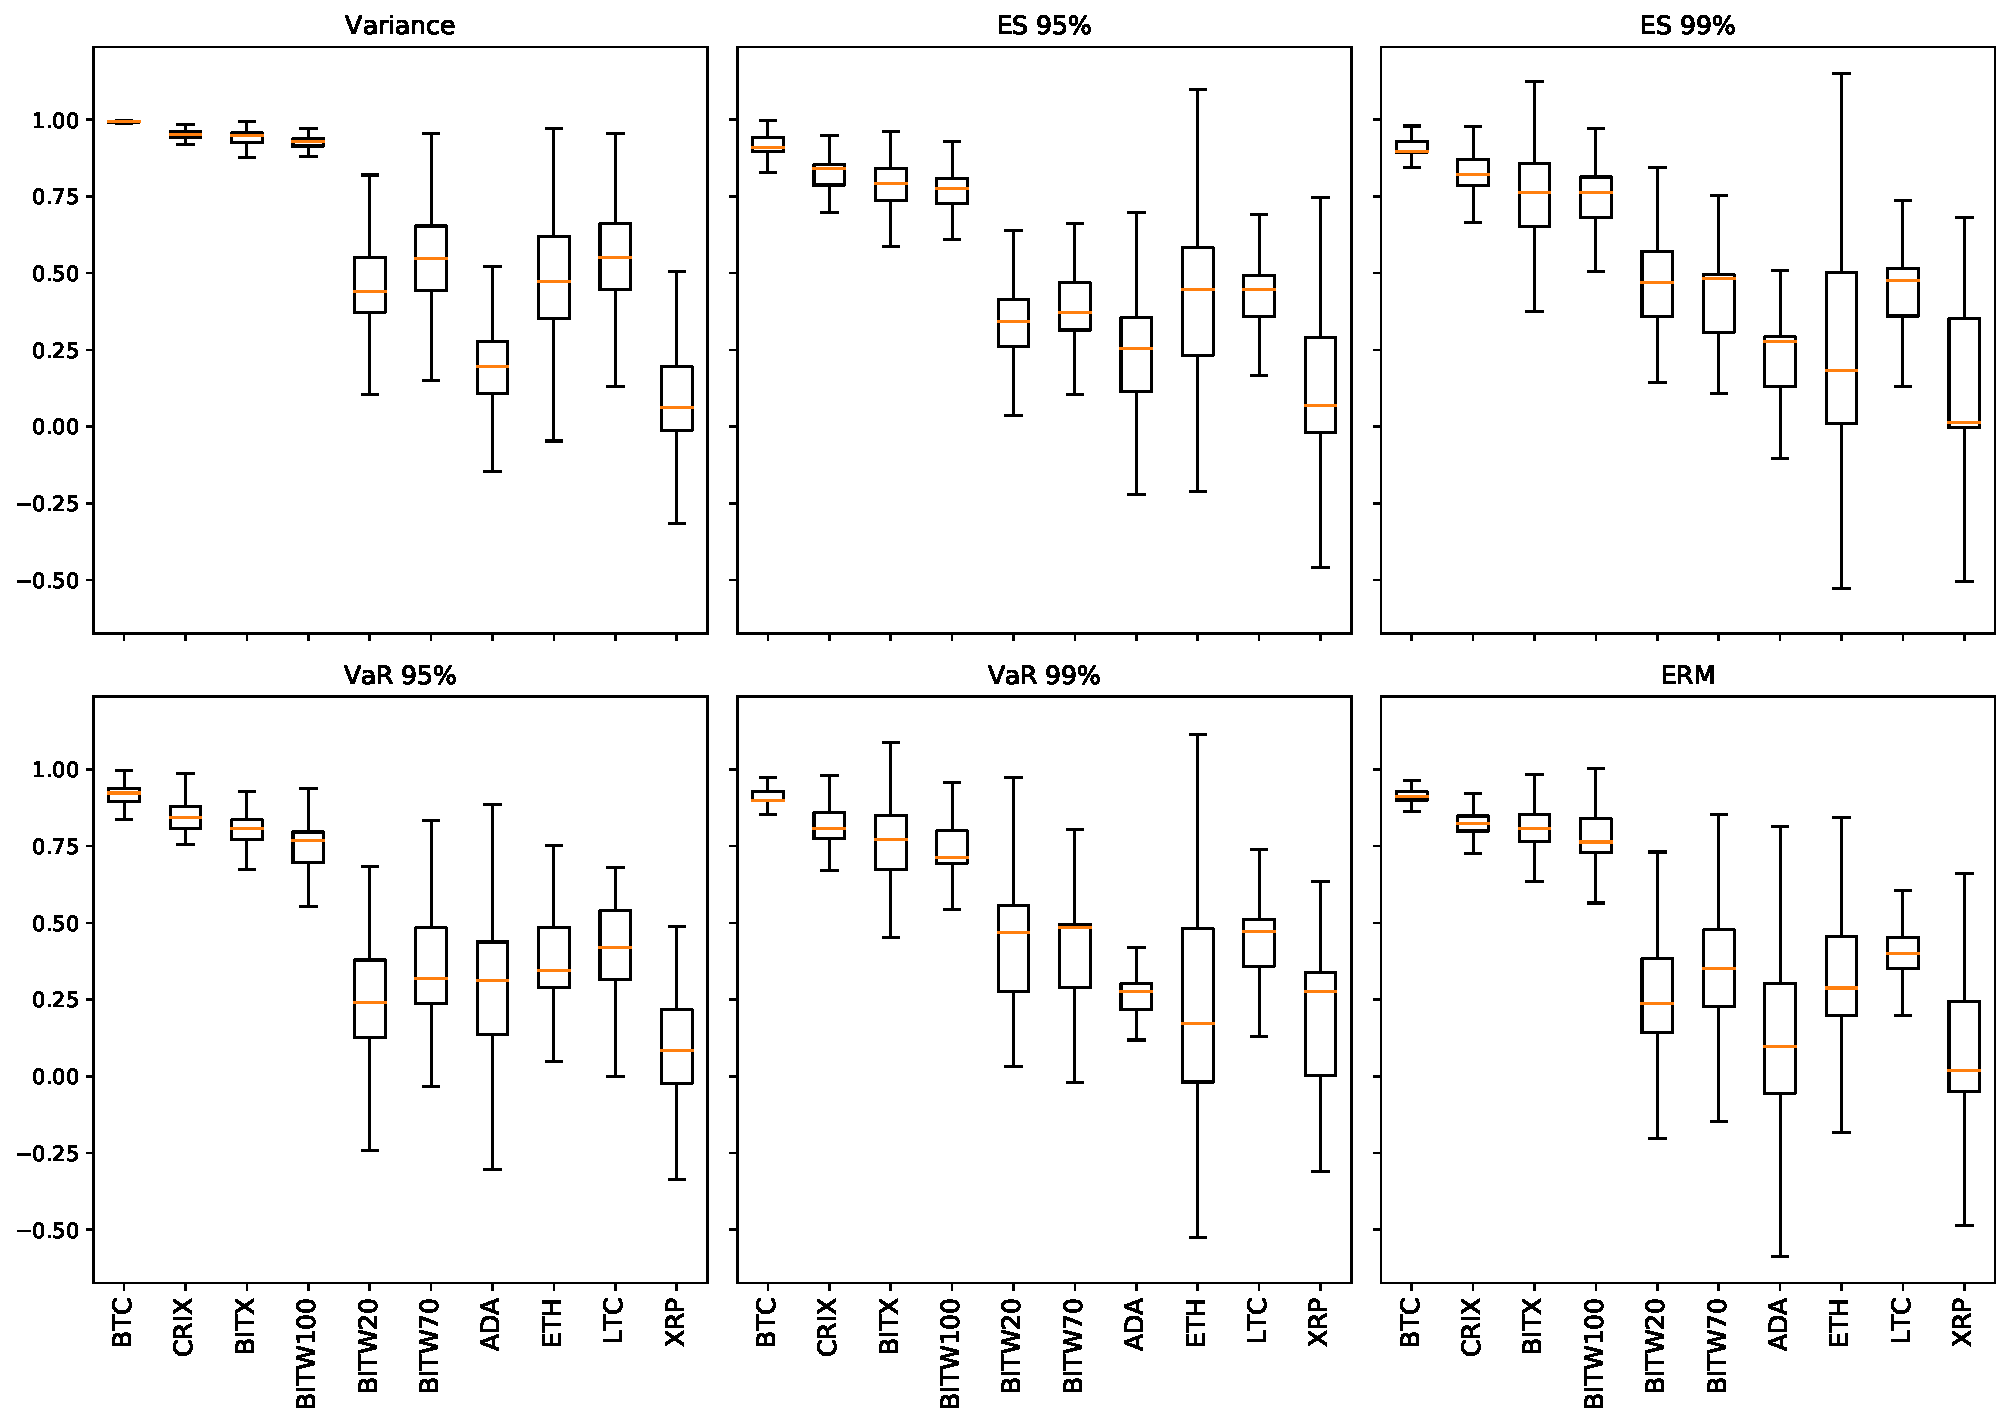
\includegraphics[width=\textwidth]{_pics/ES5_HE_boxplot.pdf}
  \caption{HE evaluated in the corresponding risk minimization objectives.
            The boxplots indicate the the median, upper quartile, lower quartile, minimium and maximum of the bootstrapped HE.
            The HE of BTC-involved spots are significantly higher than that of BTC-not-involved spots.
  \href{http://www.quantlet.com/}{\includegraphics[height=\baselineskip]{_pics/qletlogo_tr.png}} }
\label{fig:HEboxplot}
\end{figure}

%\newpage
%\begin{figure}[ht!]
%  \begin{turn}{-90}
%    \begin{minipage}{0.9\paperheight}
%      \centering
%      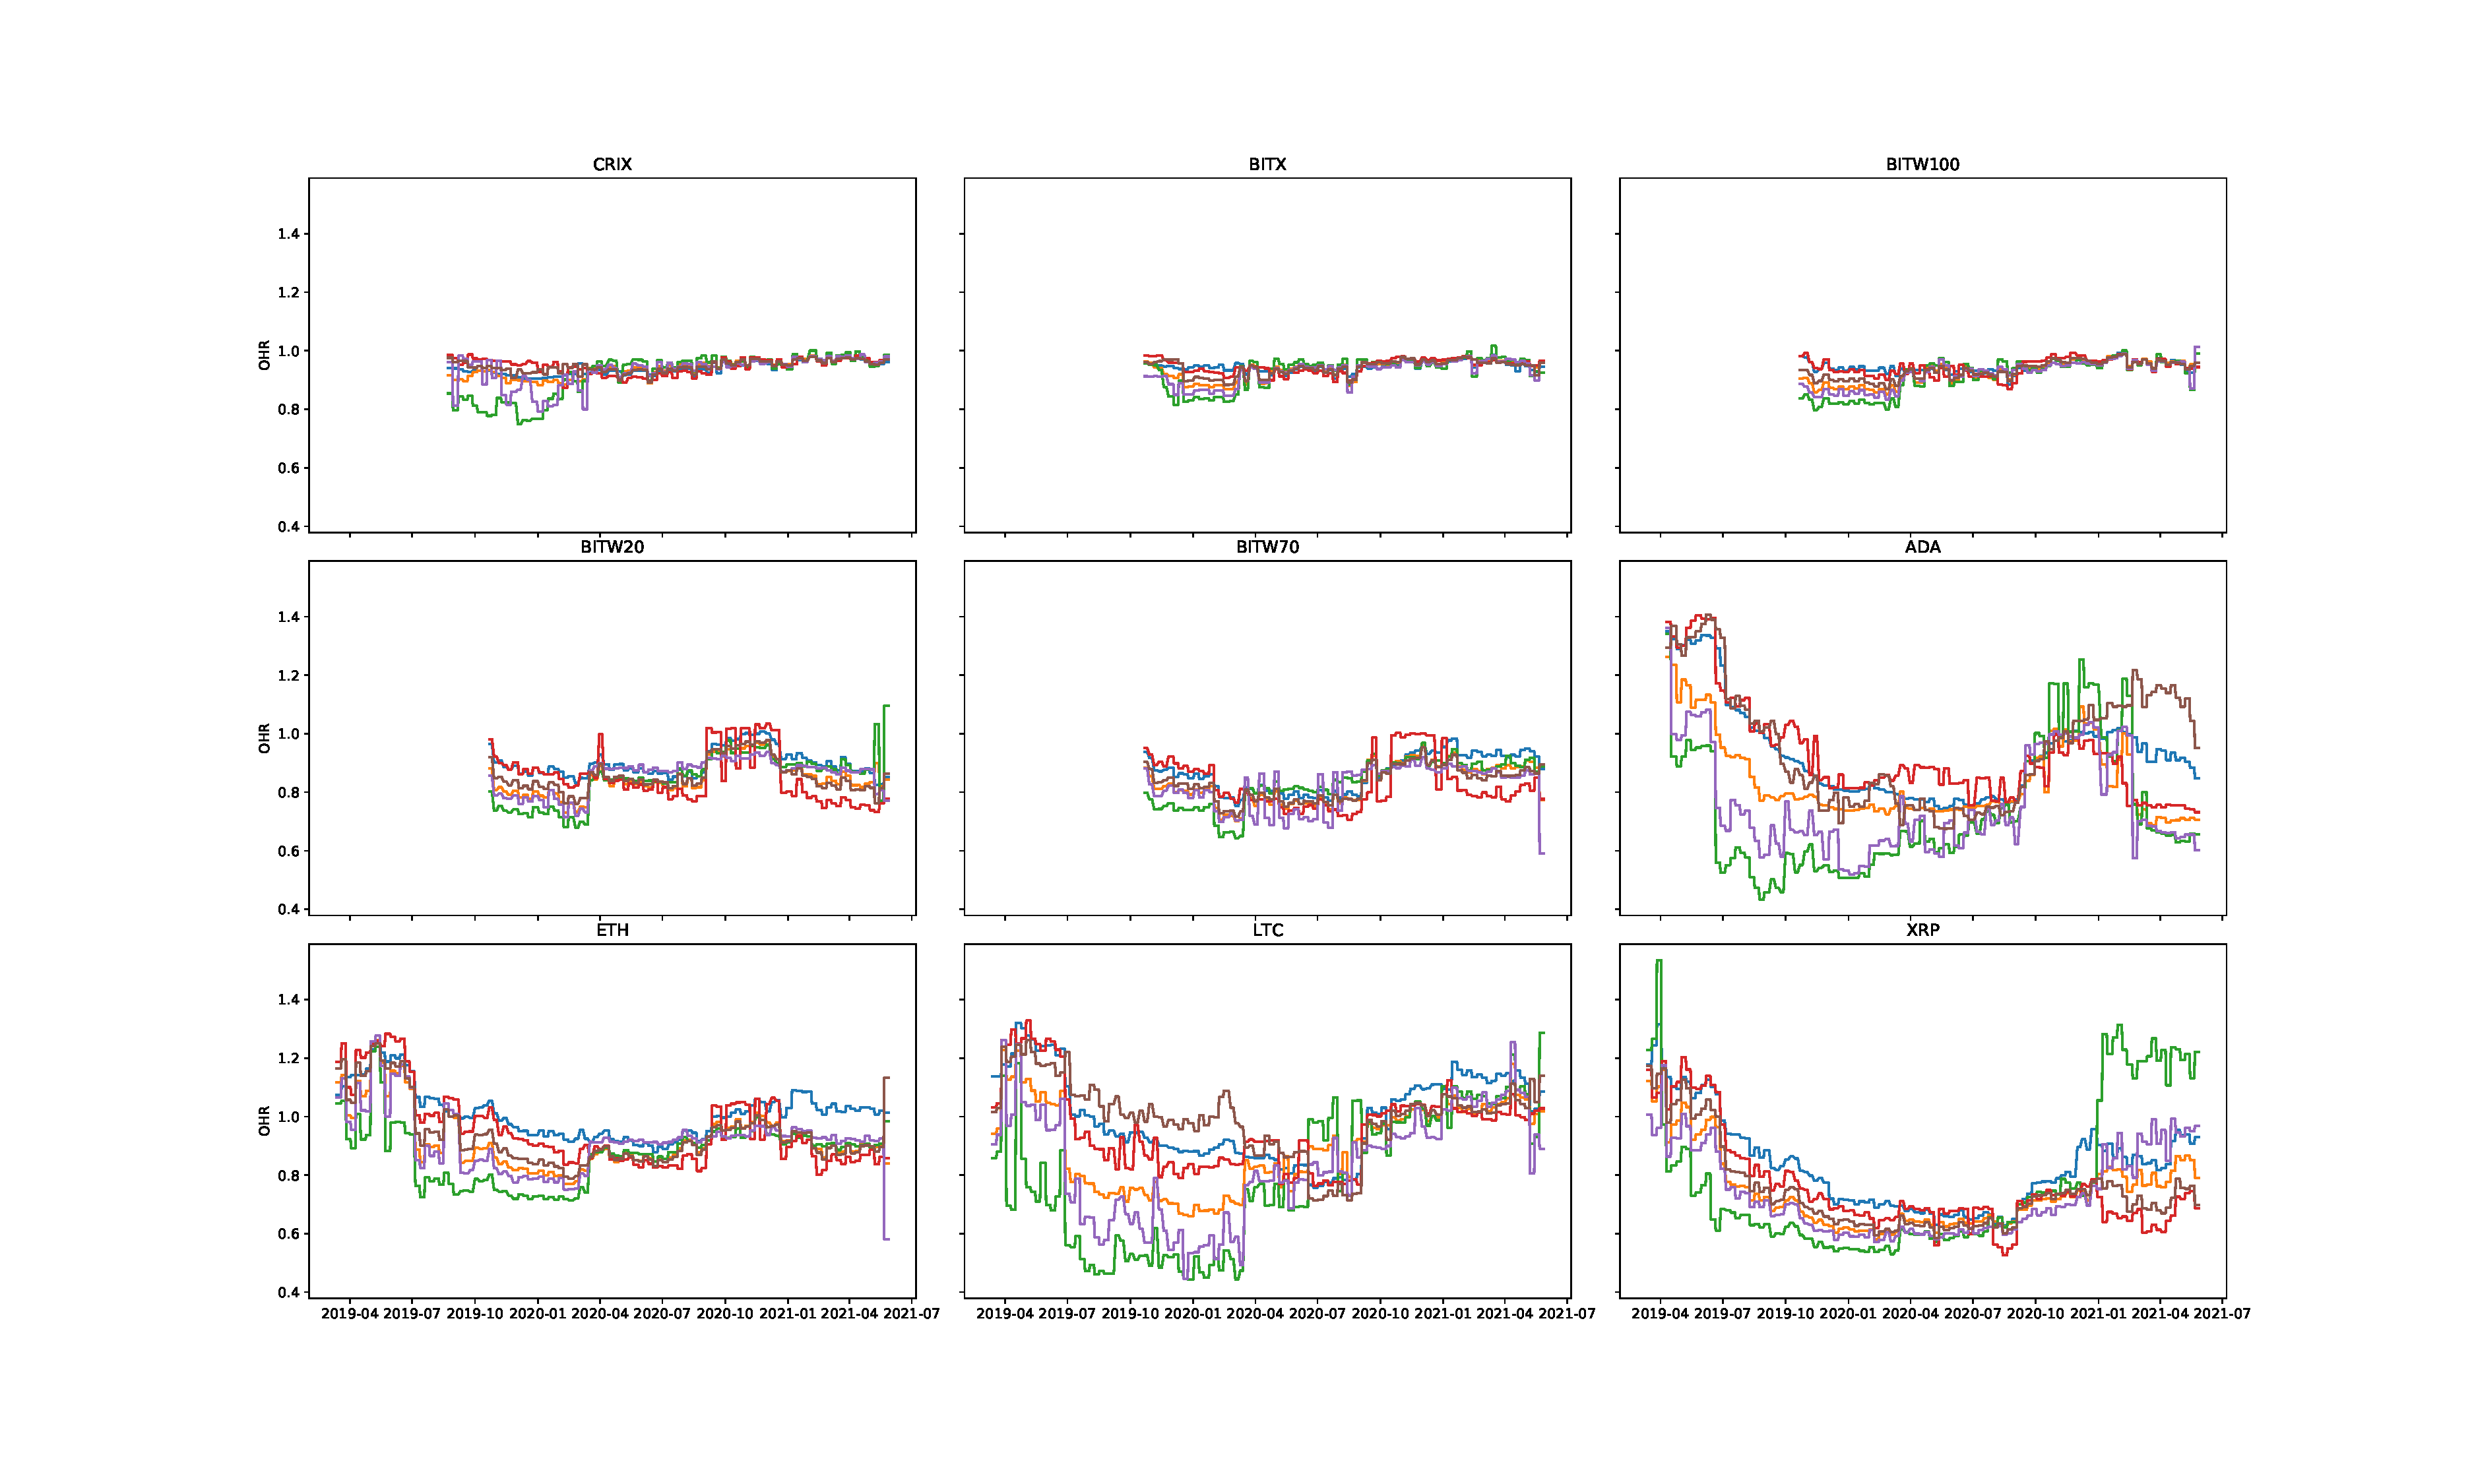
\includegraphics[angle=0,origin=c, width=0.9\paperheight]{_pics/OHRs_timeseries.pdf}
%      \captionsetup{width=0.75\paperheight}
%      \caption{ OHR time series. The \textcolor{plt1}{blue line} is OHR minimizing variance,
%                                      \textcolor{plt2}{orange line} is that of ES 95\%,
%                                      \textcolor{plt3}{green line} is that of ES 99\%,
%                                      \textcolor{plt4}{red line} is that of VaR 95\%,
%                                      \textcolor{plt5}{purple line} is that of VaR 99\%, and
%                                      \textcolor{plt6}{brown line} is that of ERM $k=10$.
%      \href{http://www.quantlet.com/}{\includegraphics[height=\baselineskip]{_pics/qletlogo_tr.png}} }
%      \label{fig:OHR-timeseries}
%    \end{minipage}
%  \end{turn}
%\end{figure}
%\newpage

